\documentclass{ctexart}
\usepackage{cite} 
\usepackage{subfigure}
\usepackage{amsmath}

\title{综述:深度神经网络在计算机视觉的应用}  
\author{韩笑}

\begin{document}
\nocite{*}

\maketitle

\tableofcontents
 
\clearpage
\begin{abstract}
计算机视觉包含图像识别、目标检测、语义分割等任务,在无人驾驶、安防、人机交互等领域应用广泛,学术界和工业界都致力于得到更加准确、高效的算法。特征提取、傅里叶变换、机器学习等传统方法虽然取得了较好的成果,但是难以实用化,而且进步空间小,发展缓慢。2012年起,以AlexNet为代表的深度学习再次引领了计算机视觉的发展潮流。虽然兴起时间不到十年,但是带来大量技术突破,相关论文浩如烟海。本文试图整理本次浪潮下深度神经网路在计算机视觉中的发展脉络,为深入研究打下基础。
\end{abstract}

\section{前言}
%背景和动机描述
\subsection{背景}
计算机视觉在生产生活中应用广泛,如无人车辆需要分析摄像头拍摄的图片以判断路况\cite{sheth2018design, cardarelli2017cooperative};安防系统比对图片数据库锁定嫌疑人\cite{li2015convolutional,yang2016wider,jiang2017face,farfade2015multi};体感游戏对用户姿态分析实现人机交互\cite{belagiannis2017recurrent,lifshitz2016human}。这些需求要求更加迅速、准确、可靠的计算机视觉算法。传统的计算机视觉算法一般通过特征工程、滤波器、机器学习等方法\cite{zuo2018learning,jordan2015machine,lison2015introduction,meyer2015support},取得了一定的成果,但是发展陷入了瓶颈,到大规模应用还有很大差距。近些年兴起的深度学习在计算机视觉领域掀起轩然大波,占据各个视觉竞赛榜首\footnote{http://cocodataset.org}\footnote{http://www.image-net.org/}\footnote{https://www.kaggle.com/},相关算法层出不穷,论文数量与日俱增,性能逐步提高。

但是我们也看到,深度学习在部分计算机视觉问题上研究不充分,如三维计算机视觉\cite{song2015sun,song2016deep,whelan2015real}、复杂条件下的识别\cite{wu2016robust}等;除此之外,深度学习的发展也带来了意想不到的问题,如视觉攻防、信息安全\cite{whelan2015real,rao2015computer}等;深度学习在其他领域的发展也为计算机视觉带来新思路,如生成对抗网络(GAN)\cite{faubel2016cilia,goodfellow2014generative}在视觉领域的应用。这些新领域新问题新思路有助于得到更加全面高效安全的计算机视觉算法。

\subsection{动机}
计算机视觉领域发展迅猛,每年的会议期刊应接不暇,顶会文章就有数千篇。对于初学者,如何在这些年万余篇论文中把握住计算机视觉的发展方向是个难题。本人也是该领域的初学者,希望通过整理最近阅读的论文、博客、代码等学习资料,浅显的归纳总结计算机视觉的成熟经验,对当下热点做一些前瞻性预测,帮助自己和同行更好的进行研究。


\section{深度神经网络}
深度神经网络包括卷积神经网络和循环神经网络。卷积神经网络一般应用于计算机视觉,循环神经网络一般应用于自然语言处理。近年来,两者发展都很快,并且相互借鉴。
\subsection{卷积神经网络}
\paragraph{LeNet}\cite{lecun1998gradient}由Yann LeCun于1998年提出,是第一种实用的卷积神经网络,广泛用于手写字符识别。如图\ref{fig:lenet},LeNet网络结构简单,仅包括7层,但是包含了深度学习的基本模块:卷积层、池化层、全连接层,是所有卷积神经网络的基础。LeNet在minst数据集上取得了较好的结果,但是限于硬件算力与软件算法限制,没有应用于更加复杂的计算机视觉问题。
\begin{itemize}
\item 输入层的大小为32*32*3(三通道)
\item C1是卷积层,使用6个大小为5*5的卷积核,得到28*28*6的特征图
\item S2是池化层,步长为2,得到14*14*6的特征图
\item C3层是卷积层,通过对S2的输出特殊组合,得到10*10*16的特征图
\item S4是池化层,得到5*5*16的特征图
\item C5是卷积层,使用120个5*5的卷积,得到1*1*120的特征图
\item F6是全连接层,有84个节点
\item 输出层是全连接层,有10个节点(代表数字0-9)
\end{itemize}
\begin{figure}
    \centering
    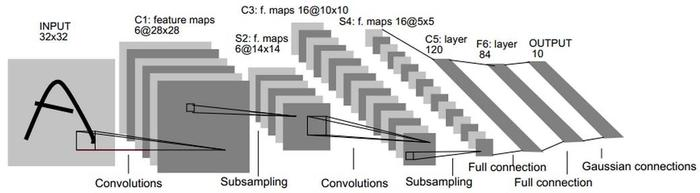
\includegraphics[width=0.7\linewidth]{AI/figures/LeNet.jpg}
    \caption{LeNet}
    \label{fig:lenet}
\end{figure}

\paragraph{AlexNet}\cite{krizhevsky2012imagenet}由Hinton及其学生于2012年提出,夺得当年ILSVRC比赛冠军,其错误率远低于已有算法。如图\ref{fig:alexnet},AlexNet在现有深度神经网络上做了大量改进,包括:使用ReLU\cite{glorot2011deep}代替Sigmoid作为激活函数,解决了神经网路深层梯度消失问题;使用Dropout\cite{srivastava2014dropout,tinto1975dropout}避免过拟合;用最大池化\cite{nagi2011max}取代平均池化,提高特征丰富性;提出局部响应归一化(Local Respone Normalization,LRN)层,增强模型泛化能力;使用CUDA和双路并行网络设计,显著加速训练;采用数据增强,减小过拟合、提高泛化能力。
\begin{figure}
    \centering
    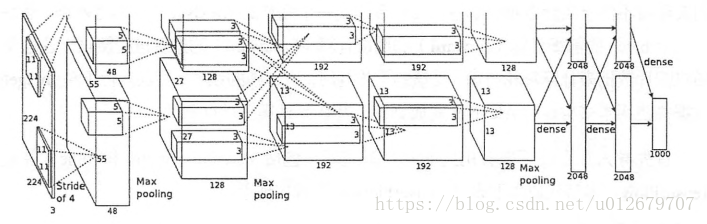
\includegraphics[width=0.7\linewidth]{AI/figures/AlexNet.png}
    \caption{AlexNet}
    \label{fig:alexnet}
\end{figure}

\paragraph{GoogLeNet}\cite{szegedy2015going}由Google公司于2014年首次提出,有多个升级版本。为有效增加模型深度(网络层数)和宽度(神经元数量),GoogLeNet提出多点创新:用多个1*1、3*3、5*5的小卷积核替代7*7的大卷积核;取消全连接层;在网络中大量使用Inception架构;增加辅助分类器。与AlexNet相比,GoogLeNet大幅增加了网络深度,同时减少了计算量和参数。

\paragraph{VGG}\cite{simonyan2014very}由Oxford Visual Geometry Group于2014年提出,和GoogLeNet一起在当年ILSVRC竞赛大放异彩。VGG比GoogLeNet参数多,但是在迁移到其它领域表现较优,常被其他领域用作基础网络。VGG结构简洁,卷积层均采用3*3的卷积核,池化层均采用2*2最大池化。

\paragraph{ResNet}\cite{he2016deep}即残差网络,由何凯明等人与2015年提出,获得当年ILSVRC多个视觉任务冠军,随即得到工业界和学术界的认可。在残差网络之前,深度神经网路一般不超过20层,更深的网络无法避免梯度消失等问题,难以训练。何凯明等人创造性的提出残差结构,打破顺序连接的惯例,将浅层输出跳跃式的输入深层,同时采用批标准化(Batch Normalization)\cite{ioffe2015batch}防止过拟合。通过这些改进,ResNet可以轻易超过上百层并且可以有效训练。残差网络的设计思路还被广泛应用于其他深度学习领域,均取得了较好的效果。

\subsection{循环神经网络}
循环神经网络(Recurrent Neural Network, RNN)主要用于处理上下文相关的问题,如自然语言处理。存在一类问题,其输入数据是一个序列,具有上下文依赖性。由于卷积神经网络前一个输入和下一个输入没有关联,处理此类问题效果不佳。而循环神经网络正是为了处理这类问题设计的,具有重复的结构。

\section{计算机视觉现状}
%做什么,怎么做,比较分析

随着深度神经网络的蓬勃发展,研究人员将其引入计算机视觉各子任务,如图像识别、目标检测、语义分割、人体姿态检测等,均取得了远超以往水平的成果。本章节从图像识别、目标检测、语义分割、实例分割、人体姿态检测这5个方面介绍现有技术的发展。

\subsection{图像识别}
图像识别任务需要将图片归类到给定种类中某一个。自2012年AlexNet在多个视觉竞赛中夺冠,深度神经网络就开始统治图像识别领域。此后,图像识别的研究集中于改进深度神经网络结构,涌现出GoogLeNet、VGG、ResNet等网络,在网络深度、卷积核、浅层信息利用等方面取得了很多成果,将图像识别推向实用化。同时,图像识别也是其他计算机视觉任务的基础,优秀的图像识别网络常被当作其他视觉任务的基础网络;GoogLeNet、ResNet的设计思路被广泛用于其他网络设计中。

\subsection{目标检测}
目标检测(object detection)任务需要识别图片中不同物体的种类,并且用矩形框标出物体的位置,如图\ref{fig:目标检测}。卷积神经网络在图像识别上取得巨大突破后,研究人员开始将其应用在目标检测中。现有的目标检测算法可以分为one-stage和two-stage两类。
\begin{figure}
    \centering
    \subfigure[]{
        \begin{minipage}[t]{0.45\linewidth}
        \centering
        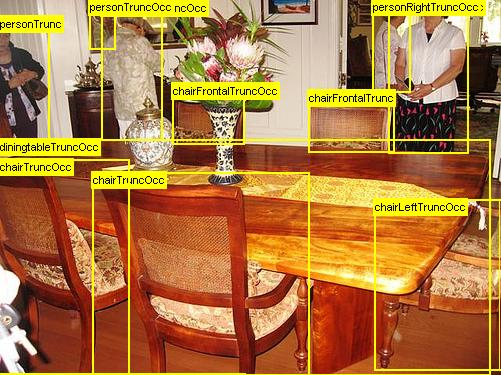
\includegraphics[width=0.8\linewidth]{AI/figures/目标检测-1.jpg}
        \end{minipage}
    }
    \subfigure[]{
        \begin{minipage}[t]{0.45\linewidth}
        \centering
        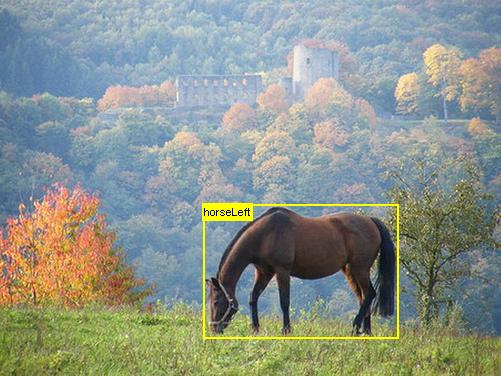
\includegraphics[width=0.8\linewidth]{AI/figures/目标检测-2.jpg}
        \end{minipage}
    }
    \caption{目标检测}
    \label{fig:目标检测}
\end{figure}

\subsubsection{two-stage算法}
two-stage算法将目标检测分为两步:产生候选区域和对候选区域分类。这种思路较为直观,对应算法只需要在图像识别的基础上增加了产生候选区域模块即可。
\textbf{R-CNN}\cite{girshick2014rich}算法是深度神经网络在目标检测领域最早的实践,其主要过程分为四步:首先利用Selective Search算法在图像中生成1000-2000个候选区域;然后将其归一化为统一尺寸后送入卷积神经网络提取特征;神经网路输出的特征送入每一类对应的SVM二分类器分类;最后使用回归器精细修正候选框位置。R-CNN的每个候选框都需要归一化后送到神经网路提取特征,计算量大。

\textbf{SPP-net}\cite{he2015spatial}简化了R-CNN的第二步。先将单张图片送入神经网路提取特征,得到一张特征图,随后对每个候选框区域空间金字塔池化(Spatial Pyramid Pooling,SPP),得到多个固定大小的特征向量。算法核心是空间金字塔池化,它利用特殊的池化层将不同大小的特征图转化为相同大小的特征向量,效果优于暴力拉伸缩放。
\textbf{Fast R-CNN}\cite{girshick2015fast}借鉴SPP-net,做了两点改进:1.简化空间金字塔池化为ROI(Region of interest) pooling。ROI是表示预选框位置的五维矩阵,包括图片索引和左上角右下角坐标。pooling过程如图\ref{fig:ROI},根据ROIs和前层得到的特征图,将候选框分割为预设尺寸的小块;寻找每个小块的最大值;最终得到输出矩阵。2.利用神经网络取代原先的类别分类和位置回归。为此需要多任务损失函数。
\begin{figure}
    \centering
    \subfigure[]{
        \begin{minipage}[t]{0.25\linewidth}
        \centering
        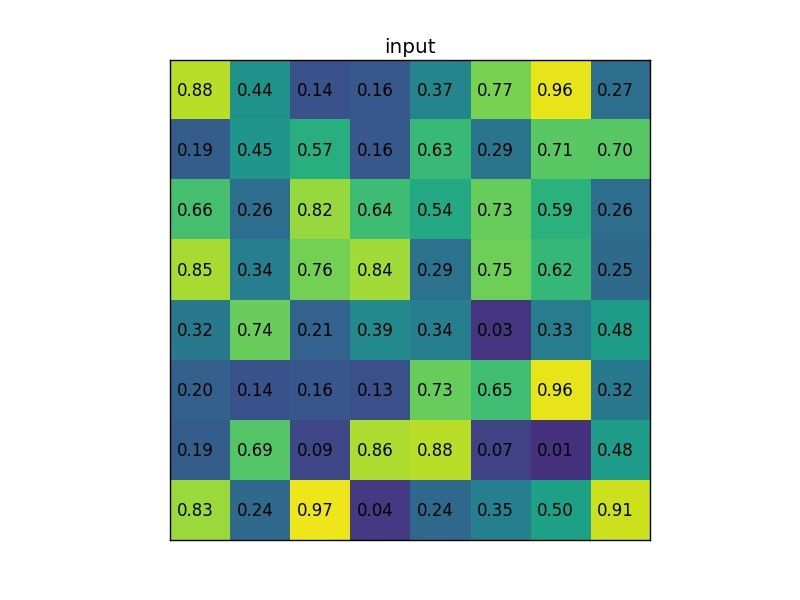
\includegraphics[width=1in]{AI/figures/ROI-1.jpg}
        \end{minipage}
    }
    \subfigure[]{
        \begin{minipage}[t]{0.25\linewidth}
        \centering
        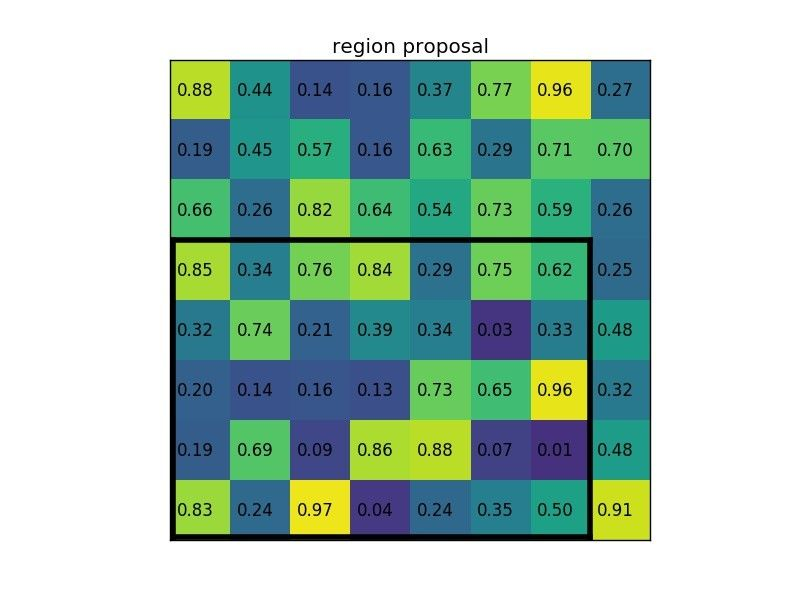
\includegraphics[width=1in]{AI/figures/ROI-2.jpg}
        \end{minipage}
    }
    \subfigure[]{
        \begin{minipage}[t]{0.25\linewidth}
        \centering
        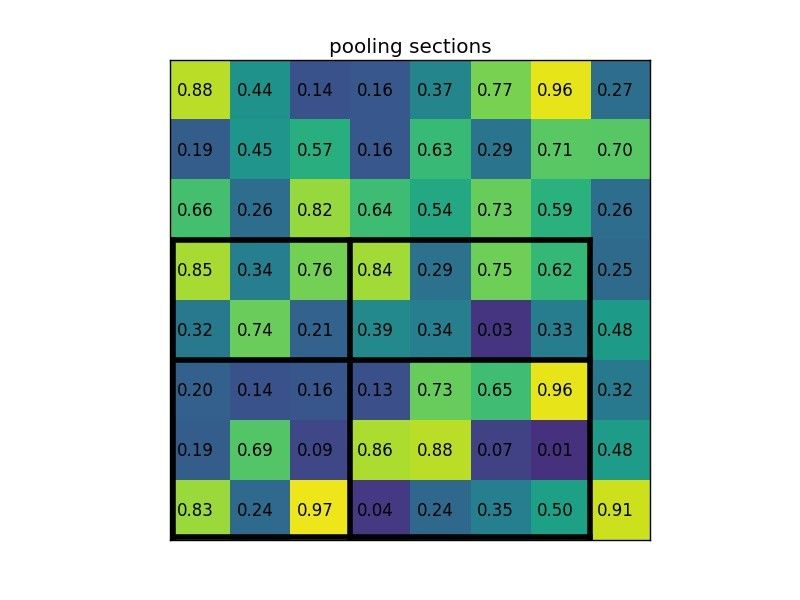
\includegraphics[width=1in]{AI/figures/ROI-3.jpg}
        \end{minipage}
    }
    \subfigure[]{
        \begin{minipage}[t]{0.25\linewidth}
        \centering
        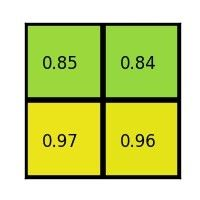
\includegraphics[width=1in]{AI/figures/ROI-4.jpg}
        \end{minipage}
    }
    \caption{ROI pooling}
    \label{fig:ROI}
\end{figure}

从R-CNN升级到Fast R-CNN,整个算法还剩下一个瓶颈:生成候选框。\textbf{Faster R-CNN}\cite{ren2015faster}放弃了传统候选框生成算法Selective Search,设计了RPN(Region Proposal Network)。RPN的输入与ROI pooling的输入相同,而且这两层均为单层卷积层,整个算法变成全卷积结构。故对于单张图片,只需要运行一次神经网络,节省大量计算开销。RPN生成候选框的过程如下:对于特征图的每个点,生成k个anchor boxes(一般设置3种scale和3种aspect rations,共9个anchor boxes)。每个anchor box预测6个参数,2个为存在物体和不存在物体的概率,另外4个是坐标。如果送入RPN的特征图尺寸为W*H,则预测W*H*k个anchor boxes,可以通过nms等方法过滤。

\subsubsection{one-stage算法}
one-stage的解决思路是利用单个卷积神经网络,直接输出预测框的位置信息和物体类别,代表者是YOLO\cite{redmon2016you,redmon2017yolo9000}和SSD\cite{liu2016ssd}。\textbf{YOLO}将预测框和分类两个任务合并,利用利用卷积层提取信息,全连接层输出类别与位置。检测过程先将输入的图片划分为S*S个cell,每个cell负责预测中心点落在该cell的物体的类别和位置。一个cell预测B个bounding box,B个bbox共享类别概率,输出一组5*B+class\_num维结果。以B=2,class\_num=5为例,每个cell输出为:
$$
[x_1,y_1,w_1,h_1,c_1,x_2,y_2,w_2,h_2,c_2, class_1 .... class_5]
$$
YOLO另一个创新是损失函数。传统的目标检测算法中,类别是分类问题,定位是回归问题;而YOLO将两者统一为回归问题,最近预测每个类别的概率而不是二分类。

\textbf{SSD}与YOLO都采用单个神经网络实现分类定位,如图\ref{fig:SSDvsYOLO}。相对于YOLO,SSD作了以下改进:借鉴ResNet的思路,将浅层的特征图连接到最后一层,显著提高了模型的准确度,特别是对小目标的识别能力;以Faster R-CNN的Anchor Box代替YOLO的Bounding Box;网络中部分使用DeepLab提出的空洞卷积。
\begin{figure}
    \centering
    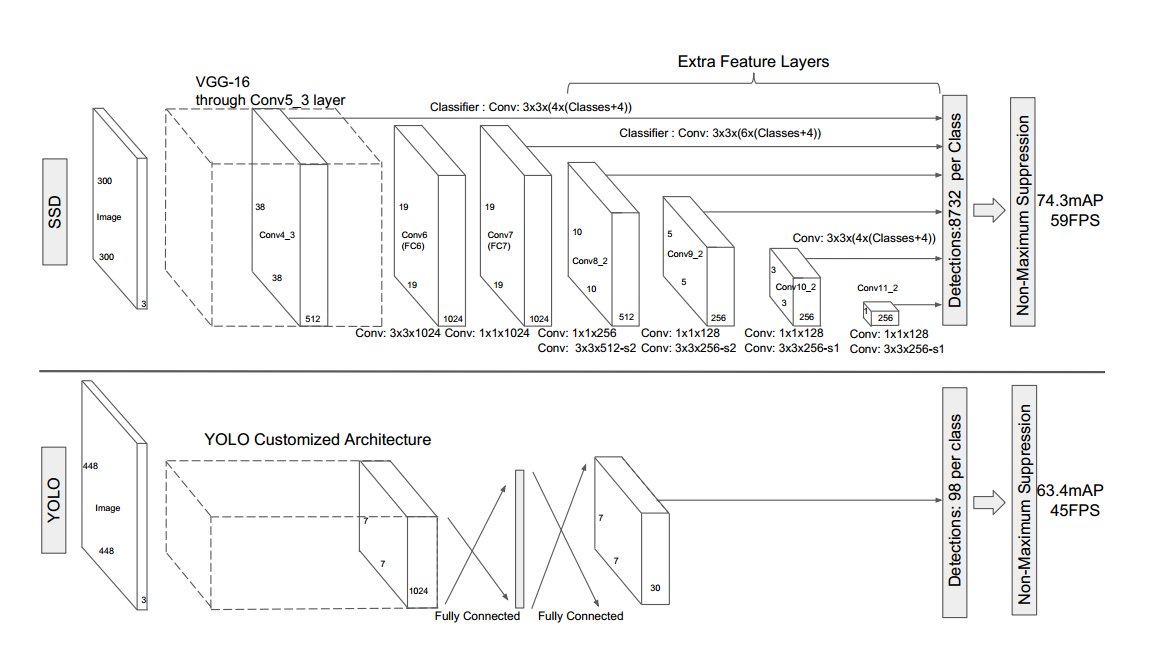
\includegraphics[width=0.7\linewidth]{AI/figures/SSDvsYOLO.png}
    \caption{SSD与YOLO}
    \label{fig:SSDvsYOLO}
\end{figure}

早期one-stage算法和two-stage算法有明显的差异,Fast R-CNN精度高速度慢,YOLO/SSD精度低速度快。但是随着研究的深入,两者的差异越来越小,改进思路趋同。Faster R-CNN可以通过减少预选框的数量,降低精度提高速度;SSD 可以增加网格数量提高精度降低速度\cite{huang2017speed}。R-CNN算法最近的改进,如Grid R-CNN\cite{lu2018grid},融入了网格思想,提高了预测精度。

\subsection{语义分割}
语义分割(Semantic Segmentation)任务需要对输入图片像素级别的分割。可以认为这是更进一步的目标检测,不再用矩形框表示位置,而是用像素点的分类。

\textbf{FCN}\cite{long2015fully}是深度学习在语义分割上的开山之作,借鉴很多现有深度神经网络结构,如图\ref{fig:FCN}。在VGG、GoogLeNet等深度神经网络中,输入图片经过大量卷积层和池化层后,得到的特征图尺寸远小于原尺度。而对于语义分割任务,小尺寸特征图不足以进行像素级别的分割。为了解决这个问题,FCN提出了上采样层结构,即将下采样层(卷积层和池化层)得到的特征图,送入上采样层(反卷积层)恢复到原有的尺寸。由于下采样层一直在减小输出的尺寸,其最后一层输出的特征图信息丢失严重,FCN将多个尺寸的特征图叠加以提高预测精度,即跳层连接(skip connections)。以FCN-16s为例,将con7得到的1*1的特征图上采样为2*2之后和pool4之后的2*2的特征图组合,得到16倍上采样(即与输入相同的尺寸的输出),与原始的FCN相比,预测精度显著提高。FCN将整个网络分为下采样和上采样两部分,此后的语义分割模型大多按照这个思路设计、改进。
\begin{figure}
    \centering
    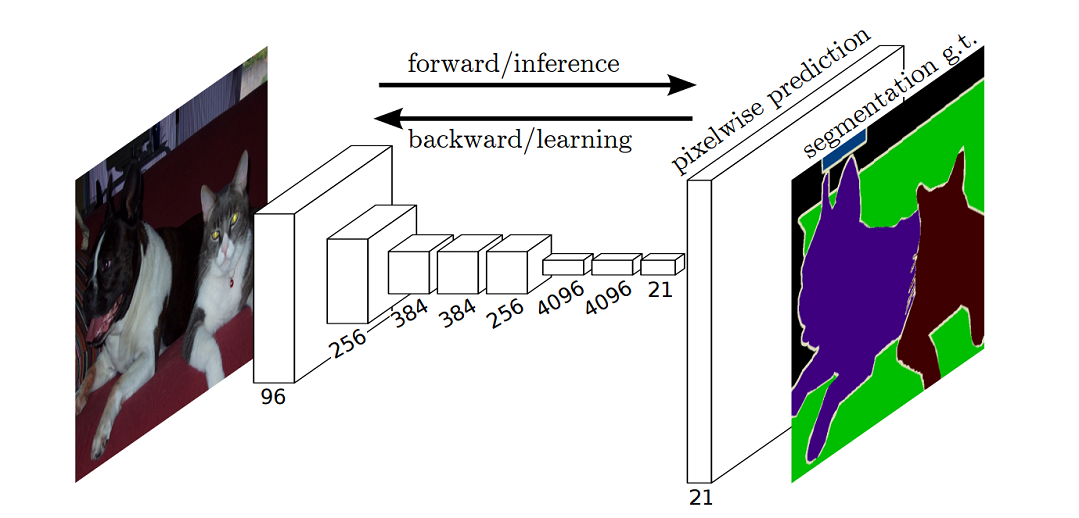
\includegraphics[width=0.7\linewidth]{AI/figures/FCN.png}
    \caption{FCN}
    \label{fig:FCN}
\end{figure}

FCN存在很多问题,它虽然结构对称,但是从参数角度,其下采样层参数占网络总参数的90\%以上。\textbf{SegNet}借鉴FCN的思路:先下采样,后上采样,并将上采样部分称为编码,下采样称为解码。但是与FCN采用skip connections融合浅层信息不同,SegNet将不同卷积层的输出连接到反卷积层的不同位置,如图,这也有利于减小上采样和下采样的参数差距。此外,SegNet还改进了池化层,编码部分的池化层结果保存对应坐标,用于解码还原,保留信息,提高准确率。如图,池化后的6对应一个坐标(1,1),8对应(1,3),在对应的decoder层,将池化结果n*n还原为2n*2n,每个数字还原到对应的位置,其他位置置0(靠反卷积层学习这些位置的数值)。

之前的语义分割,比如FCN,主要依靠池化层进行下采样,降低图像的像素并且增大感知野,之后利用反卷积上采样将图像恢复到原来的尺寸,并且将卷积过程中的不同尺寸的特征图结合提高性能;SegNet将网络分为编码和解码(encoder and decoder)两部分,将编码后得到的特征图与指定解码部分连接,并记录编码部分池化层位置以提高信息利用率。这些算法都遵循一个思路:利用池化减小图像尺寸以增大感受野,随后上采样还原图像尺寸。

利用池化层增大感知野会造成图像尺寸减小、导致信息丢失,而上采样不能完全恢复这些信息。\textbf{DeepLab、Dilated Convolutions}\cite{yu2015multi,chen2018deeplab}等提出了空洞卷积。利用空洞卷积替代池化层,既可以增大感知野,又不会减小图像尺寸。同时,DeepLab引入CRF处理神经网路得到的分割结果,使得最终结果更可靠。现在,DeepLab及其改进是语义分割任务最常见的算法。

\subsection{实例分割}
实例分割(Instance Segmentation)任务是目标检测与语义分割的结合,既需要将物体像素级别分割,又需要识别出分割后物体的类别。它与语义分割的不同之处在于是否区分属于相同类别的不同实例。例如,当图像中存在多只猫,语义分割认为所有猫所在所有像素点均属于猫;而实例分割需要区分出不同像素点分属与不同的猫。

实例分割算法往往是目标检测和语义分割现有算法的集成。\textbf{SDS}\cite{de2017semantic}在AlexNet的基础上增加了SVM,nms等方法,首次使用深度神经网络解决实例分割任务。最新研究将Faster R-CNN与FCN结合,得到\textbf{Mask R-CNN}\cite{he2017mask},效果显著提高,并且可以单独输出目标检测或者语义分割的结果。

\subsection{人体姿态检测}
人体关键点检测(Human\,Keypoint\,Detection)任务需要定位人体的关键点(一般为关节,面部五官)以表示人体姿态,也称为人体姿态估计、人体姿态检测(如图\ref{fig:keypoint}),在行为识别、人机交互、游戏、动画等领域有着很广阔的应用前景。姿态检测算法分为两大类,单人姿态估计和多人姿态估计。

也有将姿态检测分为基于检测(detection-based)的方法和基于回归(regression-based)的方法:基于检测的方法是基于热度图的,对每个关节都生成所有位置的似然热度图,选择概率最大的位置作为该关节的位置。这种方法的缺点是:1. 取概率最大值的操作是不可微分的,所以无法使用端到端的训练方法;2. 由于深度神经网络的降采样操作,热度图的分辨率远低于输入图片的分辨率,这将导致不可逆的量化误差,关节位置的精度会因此受到限制。而使用更高分辨率的热度图,会产生更多的内存和计算开销。

多人姿态估计姿态检测一般有两种方法,一种是自顶向下(Top-down),即先检测图片中人体位置,再检测出该人体的关键点,得到姿态,准确度较高但是速度慢;一种是自底向上(Bottom-up),即先检测出图片中的关键点,再分配给图中的人体,速度快但是准确性较低。



\begin{figure}
    \centering
    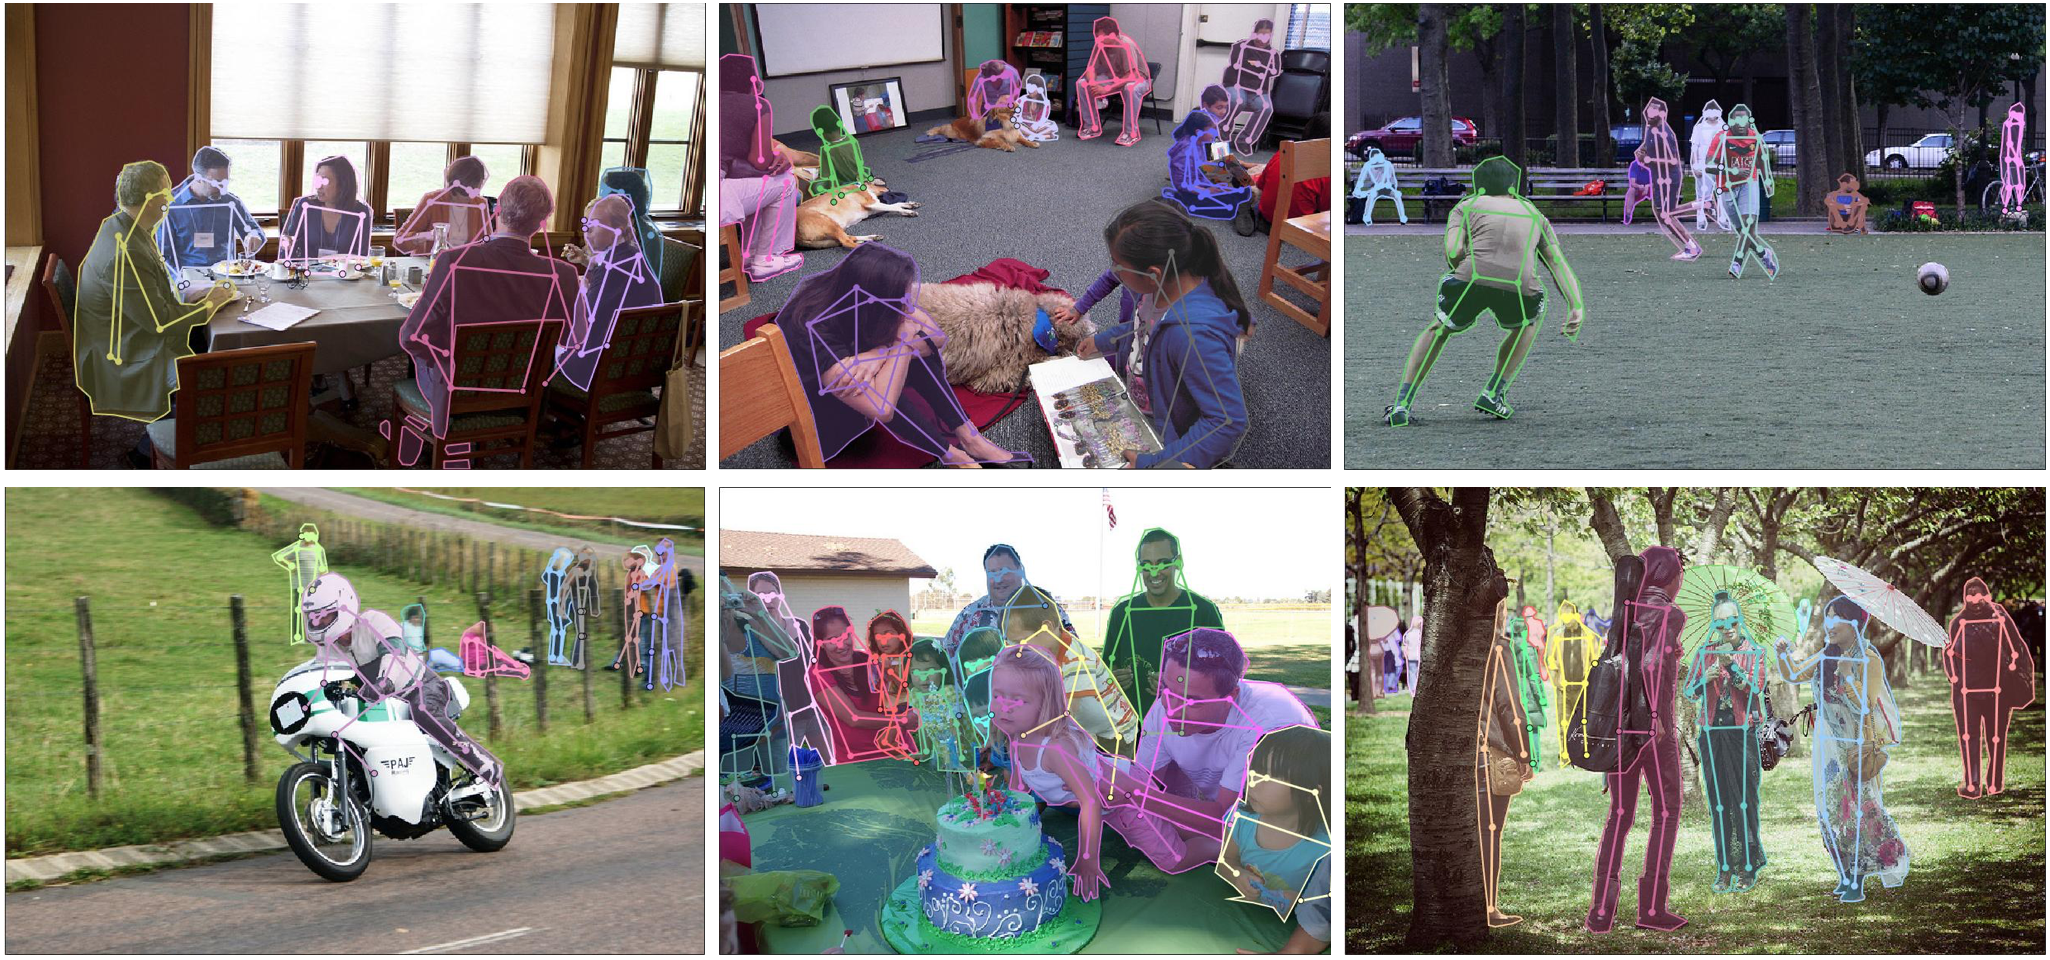
\includegraphics[width=0.7\linewidth]{AI/figures/keypoints-splash-big.png}
    \caption{人体姿态检测}
    \label{fig:keypoint}
\end{figure}



\section{实验与测评}
% 定性测评(主管评测),定量评价(正确率等指标)

深度神经网络的发展一直是实验创新先于理论突破。本章节总结实验与测评的相关技巧。

\subsection{实验}

\subsubsection{数据集}
COCO,ImageNet是现阶段最大最全的两个数据集,在图像识别、目标检测、语义分割领域广泛使用,是衡量算法性能的重要工具。不同的计算机视觉任务还有很多对应的数据集,如车辆识别、行人识别、艺术品等。

\subsubsection{训练}
\paragraph{end-to-end}
深度神经网络在训练上的追求。一端输入数据,一段出结果,训练过程不需要额外干预。

\subsection{测评}
在算法、模型的评估中,TP、FP、FN、TN是最基础的概念,如表\ref{tab:table1}。
\begin{table}[!htbp]  
\centering
\caption{样本分类}
\label{tab:table1}%添加标题 设置标签  
\begin{tabular}{ccc}  
\hline  
 & 正类 & 负类\\
\hline  
分类   & TP & FP\\
未分类 & FN & TN\\
\hline  
\end{tabular}  
\end{table}

在理解这些定义后,\textbf{准确率}(accuracy),\textbf{召回率}(recall),\textbf{精确率}(precision)就可以公式化表示。

\begin{align*}
Accuracy &= {\frac{TP+TN}{TP+FP+TN+FN}} \\
Precision &= {\frac{TP}{TP+FN}} \\
Recall &= {\frac{TP}{TP+FP}} 
\end{align*}

\paragraph{mAP}定义较为复杂,先介绍P-R图:制定一个类别,根据学习器下每个样本对这个类的预测结果进行排序,排在前面的是学习器认为“最可能”的正例样本,最后的是“最不可能的”.按照此顺序逐个把样本作为正例进行预测(1个正例,2个正例,…),则每次可以计算出当前的R值和P值,然后以R值为横轴、P值为纵轴记性作图.就得到了P-R图. 

通过P-R图可以定义AP(average precision),就是这个曲线下的面积,这里average,等于是对recall取平均。而mean average precision的mean,是对所有类别取平均(每一个类当做一次二分类任务)。现在的图像分类论文基本都是用mAP作为标准。使用AP会比accuracy要合理。对于accuracy,如果有9个负样本和一个正样本,那么即使分类器不做推测,直接全部判定为负样本,其accuracy也可以达到90\%。但是对于AP,recall=1处precision会低至0.1,曲线下的面积就会反映出性能。连续图中AP应该是P对R在[0,1]上的积分,实际上P-R图中的值是离散值,化为sum即可。而mAP是对所有类别的AP值的平均,也就是所有的AP值求和除以类数。

\section{计算机视觉新问题}
% 解决了哪些问题,还有哪些没解决

\subsection{3D-version}
前文介绍的计算机视觉算法都是基于2D场景,但是实际场景中,图片包含3D信息,利用额外的3D信息更准确的得到类别和位置情况。在对3D信息的利用上,有许多方法:
\begin{itemize}
\item 基于体素的卷积神经网络。从RGB-D图中得到体素信息,设计专门的神经网络处理体素。
\item 基于多视角的卷积神经网络。利用点云图分类。
\item 基于特征的深度神经网络。将3D数据转换为多维矩阵,送入神经网络。
\end{itemize}

\subsection{视觉安全问题}
随着深度神经网络的发展,安全问题浮出水面。部分研究人员开始在图片中增加噪声、干扰,达到“欺骗”神经网络的目的。由于深度神经网络在安防、身份识别等领域的广泛应用,安全问题迫在眉睫。

\subsection{强化学习在视觉中的应用}
生成对抗网络(GAN)在各类问题上均有使用,在计算机视觉领域\cite{mao2017least,mirza2014conditional,berthelot2017began,bousmalis2017unsupervised,isola2017image}也不例外。在数据生成、图片与文本结合领域有一定的应用。

\section{结论}
随着深度神经网络在计算机视觉中的广泛应用,分类、识别、定位、分割均取得了重大突破,在学术界和工业界都掀起波澜。但是我们也必须看到,深度神经网络自身的理论并不完善,实践先于理论,故在敏感领域的应用受限。本文对接下来深度学习在计算机视觉领域的发展,有3点猜测:
\begin{itemize}
\item 深度神经网络基础理论突破,提高可解释性;
\item 和其他领域的新思路结合,提高性能;
\item 结合先验知识,提高针对特定任务的专家系统性能。
\end{itemize}

\bibliographystyle{plain}
\bibliography{ref}
 
\end{document}

